\documentclass[12pt]{article}
\usepackage[utf8]{inputenc}
\usepackage[english]{babel}
\usepackage{bbding}
\decimalpoint
\usepackage[spanish]{babel}
\usepackage{amsmath}
\usepackage{amsthm}
\usepackage{amssymb}
\usepackage{graphicx}
\usepackage[margin=0.9in]{geometry}
\usepackage{fancyhdr}
\usepackage[inline]{enumitem}
\usepackage{float}
\usepackage{cancel}
\usepackage{minted}
\usepackage{bigints}
\usepackage{color}
\usepackage{xcolor}
\usepackage{subfig}
\usepackage{listingsutf8}
\usepackage{algorithm}
\usepackage{tocloft}
\usepackage[none]{hyphenat}
\usepackage{graphicx}
\usepackage{grffile}
\usepackage{tabularx}
\usepackage[nottoc,notlot,notlof]{tocbibind}
\usepackage{times}
\usepackage{color}
\definecolor{gray97}{gray}{.97}
\definecolor{gray75}{gray}{.75}
\definecolor{gray45}{gray}{.45}
\renewcommand{\cftsecleader}{\cftdotfill{\cftdotsep}}
\pagestyle{fancy}
\setlength{\headheight}{15pt} 
\lhead{Block ciphers}
\rhead{\thepage}
\lfoot{ESCOM-IPN}
\renewcommand{\footrulewidth}{0.5pt}
\setlength{\parskip}{0.5em}
\newcommand{\ve}[1]{\overrightarrow{#1}}
\newcommand{\abs}[1]{\left\lvert #1 \right\lvert}

\author{Reporte 1}
\usepackage{minted}
\setminted{
    style=emacs,
    breaklines=true
}

%Permite crear columnas en el documento
\usepackage{multicol} 
\usepackage{color}
\usepackage{comment}
\newcommand{\tabitem}{~~\llap{\textbullet}~~}
\newcommand{\subtabitem}{~~~~\llap{\textbullet}~~}

\usepackage{cmbright}                               % Font

\bibliographystyle{IEEEtran}
\begin{document}
		\begin{titlepage}
			\begin{center}
				
				% Upper part of the page. The '~' is needed because \\
				% only works if a paragraph has started.
				
				\noindent
				\begin{minipage}{0.5\textwidth}
					\begin{flushleft} \large
						
\includegraphics[width=0.3\textwidth]{../ipn.png}
					\end{flushleft}
				\end{minipage}%
				\begin{minipage}{0.55\textwidth}
					\begin{flushright} \large
						\includegraphics[width=0.7\textwidth]{../escom.png}
					\end{flushright}
				\end{minipage}
				
				\textsc{\LARGE Instituto Politécnico Nacional}\\[0.5cm]
				
				\textsc{\Large Escuela Superior de Cómputo}\\[1cm]
				
				% Title
				
				{ \huge Session 6: Operations in binary fields \\[1cm] }
				
				{ \Large Cryptography} \\[1cm]
				
				{ \Large Group: 3CM6 } \\[1cm]
				
				\noindent
				\begin{minipage}{0.5\textwidth}
					\begin{flushleft} \large
						\emph{Students:}\\
						
						\begin{tabular}{ll}
					     Nicolás Sayago Abigail\\
					     Naranjo Ferrara Guillermo\\
					     
					\end{tabular}
					\end{flushleft}
				\end{minipage}%
				\begin{minipage}{0.5\textwidth}
					\begin{flushright} \large
						\emph{Teacher:} \\
						Díaz Santiago Sandra  \\
					\end{flushright}
				\end{minipage}
				
				\vfill
				
				% Bottom of the page
				{\large March 27, 2019}
			\end{center}
		\end{titlepage}
	
	\tableofcontents
	\newpage
	
    % -------------------------------------------------------------------------------------
    %                                     TOPICS
    % -------------------------------------------------------------------------------------
    \section{Binary Fields}
        First of all it is worth to mention the definition of a field. The book "Understanding Cryptography" defines it like this.
        
        \begin{center}
            \includegraphics[width=0.8\textwidth]{Practica6/images/field.PNG}
        \end{center}
        
        Fields with a finite number of elements, are called finite fields or Galois fields, this fields are which we'll be working. 
        
        Elements of the field {$GF(p)$} can be represented by integers 0,1, . . . , p−1. The two operations of the field are modular integer addition and integer multiplication modulo p.

        In order to do arithmetic in a prime field, we have to follow the rules for integer rings: Addition and multiplication are done modulo p, the additive inverse of any element a is given by {a + (−a) = 0 mod p}, and the multiplicative inverse of any nonzero element a is defined as {$a$ * $a^{-1}$ = 1}.
        
    \section{Theory}
        Consider the following operation used to calculate each entry of the AES S-box.
        
        \begin{center}
            \includegraphics[width=0.6\textwidth]{Practica6/images/theory.png}
        \end{center}
        
        where {$b'$ = $b'_7b'_6...b'_0$} is the bitwise vector representation of {$a^{-1}$}, where {$a$ $\epsilon$ $GF(2^8)$}.
        
        \begin{enumerate}
            \item If a = 25 (in hexadecimal), use the operation above to obtain b, this value must be equal to the value stored in the AES S-box (column 5, row 2). The next table has the multiplicative inverse in {$GF(2^8)$}.
            \item Explain why the operation above is equivalent to the operations that we studied in class to generate the S-box.
        \end{enumerate}
       
       \subsection{Solving 1}
           For the table given we know that {$a^{-1}$} = {4D_{16}} = {0100 1101_2}
           
           The first thing to do is the matrix multiplication between the constant matrix and the vector that corresponding to the value of {$a^{-1}$}. 
           \[
                \left(
                    \begin{array}{rrrrrrrr}
                    1 & 0 & 0 & 0 & 1 & 1 & 1 & 1 \\
                    1 & 1 & 0 & 0 & 0 & 1 & 1 & 1 \\
                    1 & 1 & 1 & 0 & 0 & 0 & 1 & 1 \\
                    1 & 1 & 1 & 1 & 0 & 0 & 0 & 1 \\
                    1 & 1 & 1 & 1 & 1 & 0 & 0 & 0 \\
                    0 & 1 & 1 & 1 & 1 & 1 & 0 & 0 \\
                    0 & 0 & 1 & 1 & 1 & 1 & 1 & 0 \\
                    0 & 0 & 0 & 1 & 1 & 1 & 1 & 1 \\
                    \end{array}
                \right)
                \left(
                    \begin{array}{l}
                    1 \\
                    0 \\
                    1 \\
                    1 \\
                    0 \\
                    0 \\
                    1 \\
                    0 \\
                    \end{array}
                \right)
                =
                \left(
                    \begin{array}{l}
                    0 \\
                    0 \\
                    1 \\
                    1 \\
                    1 \\
                    0 \\
                    1 \\
                    0 \\
                    \end{array}
                \right)
            \]
            After that we proceed with the XOR operation derived from the sum of the vectors mod 2.
            \[
                \left(
                    \begin{array}{l}
                    0 \\
                    0 \\
                    1 \\
                    1 \\
                    1 \\
                    0 \\
                    1 \\
                    0 \\
                    \end{array}
                \right)
                +
                \left(
                    \begin{array}{l}
                    1 \\
                    1 \\
                    0 \\
                    0 \\
                    0 \\
                    1 \\
                    1 \\
                    0 \\
                    \end{array}
                \right)
                mod 2 =
                \left(
                    \begin{array}{l}
                    1 \\
                    1 \\
                    1 \\
                    1 \\
                    1 \\
                    1 \\
                    0 \\
                    0 \\
                    \end{array}
                \right)
                = 3F_{16}
            \]
            
            The resultant vector from this last operation is the value of the b vector which is the substitution value of the S-box for the input a = 25.
            
        \subsection{Explanation}
            
        
    % -------------------------------------------------------------------------------------
    %                                     INSTRUCTIONS
    % -------------------------------------------------------------------------------------
    \newpage
    \section{Programming exercises}
        In this session we will work with some common operations in several encryption algorithms . Please do the following programming exercises in teams of two students. Please only consider the following programming languages to develop the exercises: C, C++, Python, or Java.

        \begin{enumerate}
            \item Design a function to do multiplication in a binary field. This function must receive as a parameter an irreducible polynomial of degree n, m, and two a, b elements in GF(2n). Your function must return a ∗ b mod m. Please use binary representation for a, b and m. The output must be in a binary representation also. Please DO NOT USE arrays to store a, b and m.

            \item Design a function that take a binary string a and print the polynomial representation.

            \item Design a function to implement the operation in the previous section and generate the S-box.

        \end{enumerate}   

    % -------------------------------------------------------------------------------------
    %                                     PROGRAMMS
    % -------------------------------------------------------------------------------------
    \section{Multiplication in a binary field}
        
        \subsection{Function modulo\_m}
            The first thing we considered was the case where "a" was a polynomial of multiple terms. For this case we implement the function {modulo\_m} which also includes the case of a polynomial "a" of a unique term. 
            The first thing we do in this function is to validate if the grades of polynomials a and b are minor than the grade of the polynomial m.
            
            After that, in a for cycle we check bit by bit if the term corresponding to the currently evaluating bit is in "1". If that's the case we call the function binaryFieldMultiplication which returns 
            
            \begin{center}
                {corr * b modulo m}    
            \end{center}
            
            Where corr is the currently term of the polynomial a; and apply XOR to the returned value with the value we had in our variable mod after calling the function binaryFieldMultiplication.
            
            The value mod stores the addition (XOR) of each one of the of the terms of the polynomial "a" modulo m.
            
            \newpage
            \noindent\Checkmark\textbf{Code}
                    \inputminted{c++}{Code/modulo_m.c}
            
        \subsection{Funcion binaryFieldMultiplication}
            In this function is where we calculate modulo m for each one of the terms of "a" multiplied for b. Essentially we have two cases:
            
            \begin{itemize}
                \item Polynomial a is of grade 0, it means we don't have to do any left shift on b, so we return the current value of b XOR m.
            
                \item Polynomial a is of grade 1 or superior, in which case we do only one left shift over b and then a right shift over a, it is because of the recursivity of the function, so when we call the function we will pass a polynomial "b" with one left shift applied and a polynomial "a" that in essence, will tell us how many left shifts over b left to do, eventually ending in the base case that returns {a * b mod m}.  
            \end{itemize}
            
            \noindent\Checkmark\textbf{Code}
                    \inputminted{c++}{Code/binFieldMult.c}
                    
        \subsection{Binary representation}
            To represent the value of {a * b mod m} in binary we only use a for cycle where we do an AND operation between the value mod and corr, which starts in 1 and always is left shifting, so when the value of the logic operation is true, it will add a 1 to the string that contains the binary representation of mod, and when ot's false it will add a 0. 
            
            \noindent\Checkmark\textbf{Code}
                \inputminted{c++}{Code/binaryRepresentation.c}
    
    \section{Generate S-BOX}
        For this exercise we made some functions that we will explain in the next sections. Basically, the main only have the way to generate each element of the S-BOX.
        
        Each element of the S-BOX is generated with the function \textbf{elementSB}, that receive an integer, this number is an element that allow to the matrix array, the matrix array represents the table of the multiplicative inverse in GF($2^{8}$). In another words, we send the multiplicative inverse of $x$ and $y$ (positions in the table) to the function. After that we receive a number and we convert it to Hexadecimal.
        
        How a comment, we would like found a better way to get the inverse, cause literally, we capturated the table into an array of arrays. A parner said us a solution but we need to use python or something like that.

        \begin{center}
            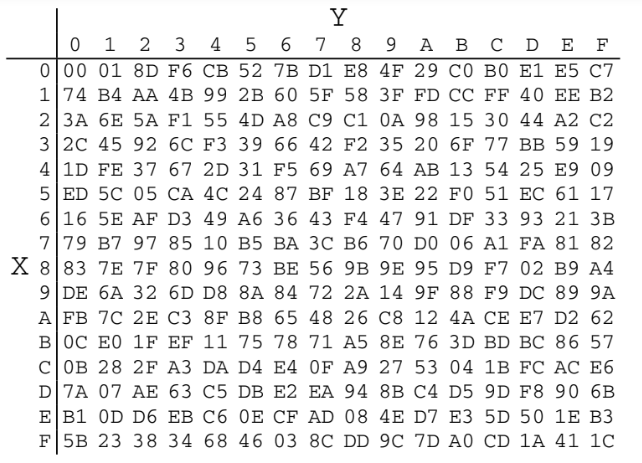
\includegraphics[width=0.8\textwidth]{Practica6/images/matrix.PNG}
            \caption{Multiplicative inverse in GF($2^{8}$)}
        \end{center}

        
        
        
        
        
        \noindent\Checkmark\textbf{Code}
            \inputminted{c++}{Code/main.c}
                    
    
    \nocite{ref2}
	    \bibliography{referencias}
        
            
\end{document}
 